%%%%%%%%%%%%%%%%%%%%%%% 部件设计 %%%%%%%%%%%%%%%%%%%%%%%%%%%%%%%%%%%%%%%%%%%%%
\chapter{部件设计}

\section{分析并发需求}

在“鲜天下”系统中,并发性的要求来自于用户的需求。后端的实现若是串行的,后端暴露给前端的API可能会由于用户请求数的增加而导致请求延时增加,服务质量下降。由此,无论是相同的API被多个用户同时调用,还是不同的API被同时调用,都需要通过并发来降低请求延时,提升用户体验。

\section{识别相应的进程和线程}

\begin{enumerate}
    \item \textbf{多用户使用同一个服务}\\以查询母订单服务为例,下图描述了三个用户同时使用母订单查询功能时,“鲜天下”平台创建进程和线程来满足用户服务的过程。
    
    \begin{figure}[htp]
        %\begin{adjustwidth}{-1.5cm}{-1cm}
        \centering
        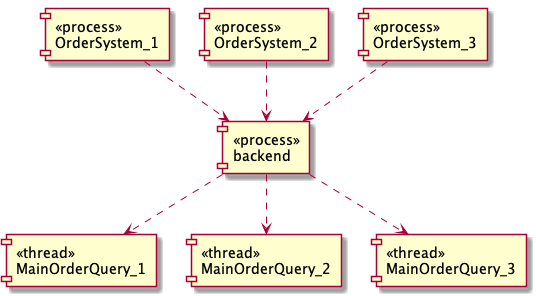
\includegraphics[width=12cm]{report/figure/component/query.png}
        \caption{多用户同时查询母订单的过程}
        \label{fig:query}
        %\end{adjustwidth}
    \end{figure}
    
    当多个用户同时进行母订单查询时,后台服务器会为每个用户的请求创建一个线程,当线程执行完查询操作时,会各自返回其结果。
    
    
    \item \textbf{多用户使用不同的服务}\\以查询子订单和查询母订单服务为例, 下图描述了两个用户分别使用查询子订单和查询母订单服务时,“鲜天下”平台创建进程和线程来满足用户服务的过程。
    \begin{figure}[htp]
        %\begin{adjustwidth}{-1.5cm}{-1cm}
        \centering
        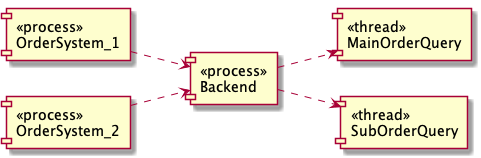
\includegraphics[width=12cm]{report/figure/component/process.png}
        \caption{多用户同时查询母订单的过程}
        \label{fig:query}
        %\end{adjustwidth}
    \end{figure}
    
    \newpage
    当多个用户同时请求不同的服务时,后台服务器会为每个用户的每个请求创建一个线程,线程执行完各自的操作后自动返回。
    
\end{enumerate}

\section{生命周期}

    如\autoref{fig:lifetime}所示,在多个用户同时调用相同(或不同)API的时候,后台会产生多个线程同时处理请求并返回相应的数据。

    \begin{figure}[htp]
        %\begin{adjustwidth}{-1.5cm}{-1cm}
        \centering
        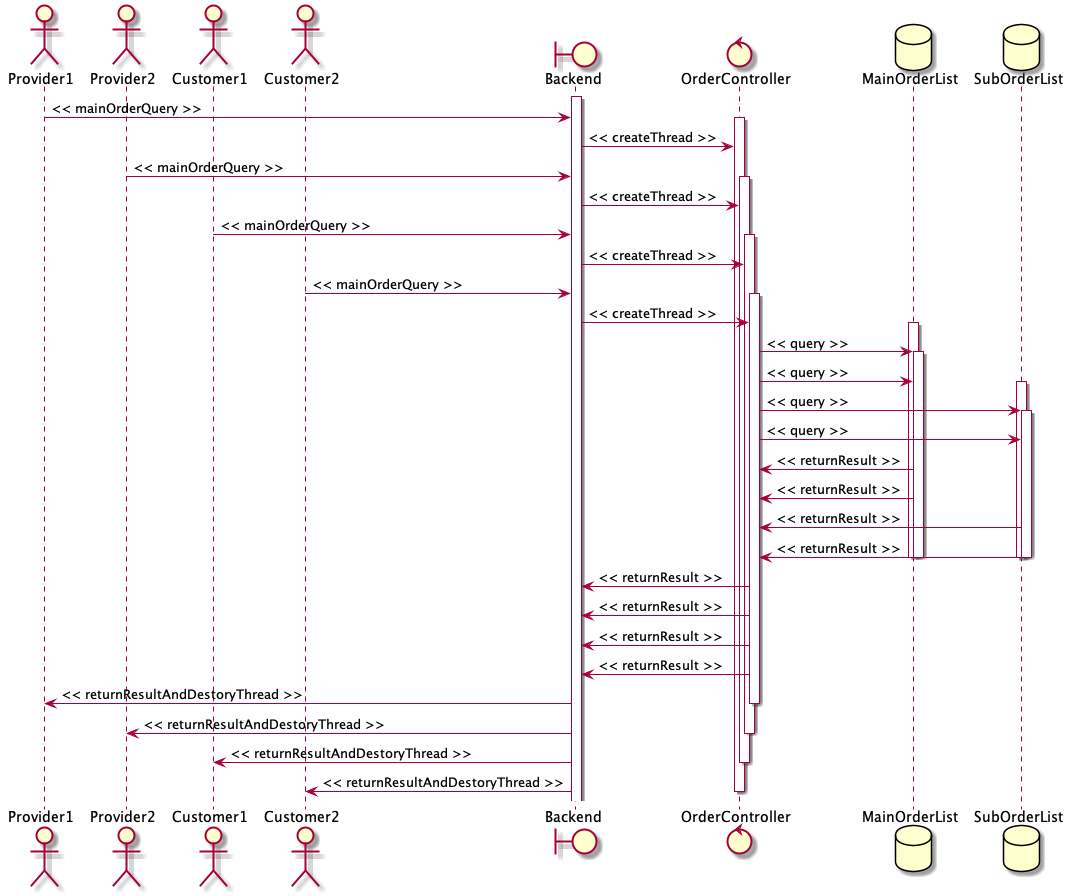
\includegraphics[width=15.5cm]{report/figure/component/lifetime.png}
        \caption{线程生命周期示意图}
        \label{fig:lifetime}
        %\end{adjustwidth}
    \end{figure}



\section{映射到现实系统}

我们的后端部署在CPU为Intel I7-7700,内存为16GB的服务器上,该CPU具备4个物理核心,8个逻辑核心,最大支持8个硬件线程。因此,后端的并发处理能够更好地利用处理器的性能,提升用户体验。